\documentclass[10pt,utf8]{beamer}

\mode<presentation> {
%  \usetheme{Boadilla}
  \usetheme{Madrid}
%	\usetheme{Fzu}
  \setbeamercovered{transparent}
}

\usepackage{palatino}
\usepackage{graphicx}
\usepackage{array}
\usepackage{color}
\usepackage{subfigure}
\usepackage{colortbl}
\usepackage{amsmath}
\usepackage{hyperref}
\usepackage{listings}
\usepackage{fancyvrb}

\setbeamertemplate{caption}{\raggedright\insertcaption\par} %turn off caption prefix ("Figure")

\title{Sanlock troubleshooting}
\author{Vojtěch Juránek}
\institute[Red Hat]{oVirt storage team}
\date{1.~12.~2020, oVirt internal}

\lstdefinestyle{bash}{
	basicstyle          = \ttfamily,
	language            = Bash,
	numbers             = left,
	numberstyle         = \small,
	stepnumber          = 1,
	numbersep           = 5pt,
	backgroundcolor     = \color{white},
	showspaces          = false,
	showstringspaces    = false,
	showtabs            = false,
	frame               = single,
	tabsize             = 2,
	captionpos          = b,
	breaklines          = true,
	breakatwhitespace   = false,
	morestring          = [b]",
	stringstyle         = \color{blue},
	keywordstyle        = \color{magenta},
	commentstyle        = \color{gray},
	identifierstyle     = \color{black},
	moredelim           = **[is][\bfseries]{`}{`},
	moredelim           = **[is][\color{magenta}]{!}{!}, 
	fancyvrb            = true,
}

\lstdefinestyle{log}{
	basicstyle          = \tiny\ttfamily,
	language            = Bash,
	numbers             = left,
	numberstyle         = \small,
	stepnumber          = 1,
	numbersep           = 5pt,
	backgroundcolor     = \color{white},
	showspaces          = false,
	showstringspaces    = false,
	showtabs            = false,
	frame               = single,
	tabsize             = 2,
	captionpos          = b,
	breaklines          = true,
	breakatwhitespace   = false,
	morestring          = [b]",
	stringstyle         = \color{blue},
	keywordstyle        = \color{magenta},
	commentstyle        = \color{gray},
	identifierstyle     = \color{black},
	moredelim           = **[is][\bfseries]{`}{`},
	moredelim           = **[is][\color{magenta}]{!}{!}, 
	fancyvrb            = true,
}


\begin{document}

\begin{frame}
    \titlepage
\end{frame}

\begin{frame}
    \frametitle{sanlock troubleshooting: TL\&DR}
        \begin{itemize}
            \item Check the storage is correctly connected and writeable.
            \item Check LVs/files \texttt{ids}, \texttt{leases}, \texttt{xleases} are writeable by \texttt{sanlock} user.
            \item Check IO on the given storage domain is not extremely slow.
            \item Check that the block size of the storage was correctly determined by vdsm.
            \item Check \texttt{/var/log/sanlock.log} for more help.
        \end{itemize}
\end{frame}

\begin{frame}
  \frametitle{sanlock}
    \begin{itemize}
        \item Distributed lock manager.
        \item Uses shared storage for exchanging information between participants.
        \item Can be used to protect any resource, not only data (e.g. keep lease for SPM host in vdsm).
    \end{itemize}

  \begin{figure}
    \centering
    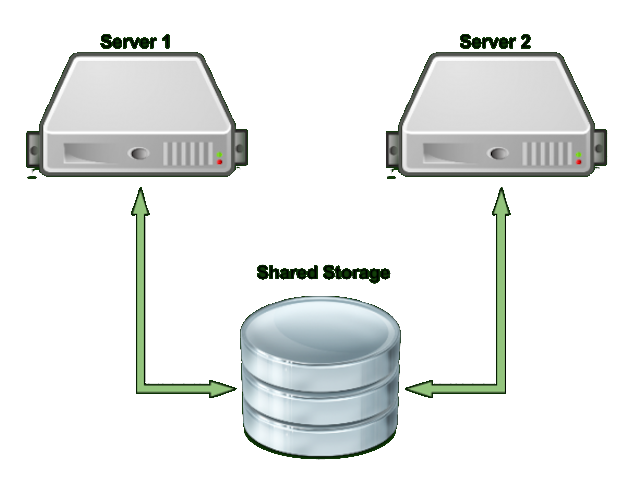
\includegraphics[height=4cm]{./img/disk-paxos.eps}
    \caption{\tiny{Source: \url{https://www.linuxjournal.com/content/high-availability-storage-ha-lvm}}}
 \end{figure}
\end{frame}

\begin{frame}
  \frametitle{sanlock leases}
    \begin{itemize}
        \item $\Delta$-leases: used for acquiring/confirming unique ID for each host (only for sanlock internal usage).
        \item Paxos leases: used for acquiring locks for resources (meaning of the lock is determined by the application).
        \item Unique host IDs are use for Paxos leases for mapping host to its disk segment.
    \end{itemize}
\end{frame}

\begin{frame}
    \frametitle{$\Delta$-Leases}
  \begin{itemize}
    \item In sanlock terminology, obtaining the $\Delta$-leases is called to join the \textit{lockspaces}.
    \item Prevents two hosts to have same ID.
    \item Lockspace size is 1~MB (for block size 512B).
    \item Maximum number of hosts is 2000.
    \item sanlock renews $\Delta$-leases every 20 seconds by writing a new time stamp into appropriate $\Delta$-lease block.
    \item Lease renewal is used also for checking if host is alive.
  \end{itemize}
\end{frame}

\begin{frame}
  \frametitle{Paxos/resource leases}
  \begin{itemize}
    \item Fast to acquire.
    \item In sanlock terminology called \textit{resources}.
    \item sanlock uses $\Delta$-lease renewals also for Paxos leases renewal in given lockspace.
  \end{itemize}
\end{frame}

\begin{frame}
  \frametitle{Lease renewal failure}
  \begin{itemize}
    \item Resource lease renewal failure: lease is released automatically by sanlock.
    \item $\Delta$-lease renewal failure: sanlock will attempt to stop or kill any process (in our case \texttt{vdsmd}) holding resource leases in the expiring lockspace.
  \end{itemize}
\end{frame}

\begin{frame}
  \frametitle{Default sanlock timeouts}
  \begin{itemize}
    \item IO timeout (\texttt{io\_timeout\_seconds}) is configurable,  by default 10 s.
    \item ID renewal 2 * \texttt{io\_timeout\_seconds}, by default 20 s.
    \item ID renewal fail/timeout (\texttt{id\_renewal\_fail\_seconds}) 8 * \texttt{io\_timeout\_seconds}, by default 80 s.
  \end{itemize}
  \vspace{0.5cm}
  \begin{itemize}
    \item \texttt{watchdog\_fire\_timeout} is 60 s (hardcoded constant).
    \item \texttt{host\_dead\_seconds} is by default 140 s (\texttt{id\_renewal\_fail\_seconds} + \texttt{watchdog\_fire\_timeout}) - host ID can be acquired by another host by this time.
  \end{itemize}
\end{frame}

\begin{frame}
    \frametitle{Usefull commands}
    \begin{itemize}
        \item \texttt{less /var/log/sanlock.log}
        \item \texttt{sanlock client host\_status}
        \item \texttt{sanlock client status}
        \item \texttt{sanlock client log\_dump}
    \end{itemize}
\end{frame}

\begin{frame}[fragile]
    \frametitle{sanlock status}
    \begin{lstlisting}[style=log]
s 78bc1ebc-4f18-4b15-a112-5524fcb198c6:1:/rhev/data-center/mnt/192.168.122.13\:_srv_data_sanlock/78bc1ebc-4f18-4b15-a112-5524fcb198c6/dom_md/ids:0
r 78bc1ebc-4f18-4b15-a112-5524fcb198c6:SDM:/rhev/data-center/mnt/192.168.122.13\:_srv_data_sanlock/78bc1ebc-4f18-4b15-a112-5524fcb198c6/dom_md/leases:1048576:8 p 5578
    \end{lstlisting}
    
    \begin{itemize}
        \item \texttt{s} - lockspace, \texttt{r} - resource
        \item name of lockspace
        \item local host identifier in lockspace or resource name
        \item path to storage to use for leases
        \item offset on path (bytes)
        \item in case of resource there can be leader version and/or \texttt{SH} in case of shared mode
    \end{itemize}
\end{frame}

\begin{frame}
    \frametitle{Lockspace/resource options}
    \begin{itemize}
        \item \texttt{lockspace\_name:host\_id:path:offset}
        \item \texttt{lockspace\_name:resource\_name:path:offset}
        \item \texttt{lockspace\_name:resource\_name:path:offset:leader\_version}
        \item \texttt{lockspace\_name:resource\_name:path:offset:SH}
    \end{itemize}
    
    \vspace{0.5cm}
    
    E.g.
    \begin{itemize}
        \item \texttt{sanlock client add\_lockspace -s test:1:/dev/loop0:0}
        \item \texttt{sanlock client acquire -r test:res:/dev/loop0:1048576 -p 29755}
    \end{itemize}
\end{frame}

\begin{frame}[fragile]
    \frametitle{sanlock from cmd line: full example}
    \begin{lstlisting}[style=bash]
qemu-img create -f raw /var/tmp/test/sanlock.img 1G
losetup --find --show /var/tmp/test/sanlock.img
sanlock daemon -w 0
sanlock client init -s test:0:/dev/loop0:0
sanlock client add_lockspace -s test:1:/dev/loop0:0
sanlock client init -r test:res:/dev/loop0:1048576
sanlock client command -c /bin/sleep 600 &
sanlock client acquire -r test:res:/dev/loop0:1048576 -p 29755
sanlock client release -r test:res:/dev/loop0:1048576 -p 29755
sanlock client rem_lockspace -s test:1:/dev/loop0:0
sanlock shutdown
losetup -d /dev/loop0
rm -f /var/tmp/test/sanlock.img 
    \end{lstlisting}
\end{frame}

\begin{frame}
    \frametitle{sanlock in vdsm}
    \begin{itemize}
        \item Each oVirt host has to join the lockspace (hold $\Delta$-lease) during activation.
        \item For each SD is one lockspace, lockspace name is SD ID.
        \item SPM host holds resource lease.
        \item Host can hold other resource leases (e.g. when running HA VM), but in many cases host doesn't hold and resource lease.
        \item When there is a problem with the storage, vdsm is not killed by sanlock, unless host/vdsm holds a lease. % e.g. https://bugzilla.redhat.com/1896215
    \end{itemize}
\end{frame}

\begin{frame}
    \frametitle{sanlock in vdsm metadata}
    SD metadata related to sanlock:
    \begin{itemize}
        \item \texttt{ids} - contains $\Delta$-leases
        \item \texttt{leases} - special/reserved resource leases (lease for SPM)
        \item \texttt{xleases} - user/external leases (e.g. leases for HA VMs). Also contains mapping between lease name and its offset in \texttt{leases}. When corrupted, can be rebuild by \texttt{vdsm-tool rebuild-xleases}
        \item Currently \texttt{io\_timeout\_seconds} cannot be change in vdsm, i.e. sanlock uses its default value of 10 s.
        \item In the future will be configurable, see \color{blue}\href{https://gerrit.ovirt.org/\#/q/project:vdsm+branch:master+topic:io-timeout}{vdsm io-timeout topic branch}\color{black}
    \end{itemize}
\end{frame}

\begin{frame}
  \frametitle{sanlock in vdsm code}
  Two main modules related to sanlock:
    \begin{itemize}
        \item \texttt{clusterlock} module (sanlock initialization, obtaining cluster lock and resource leases)
        \item \texttt{xlease} modules
    \end{itemize}
\end{frame}

\begin{frame}[fragile]
    \frametitle{vdsm udev rule for sanlock}
    \begin{lstlisting}[style=bash]
ENV{DM_LV_NAME}=="ids|leases|xleases", MODE:="0660", OWNER:="@VDSMUSER@", GROUP:="@SNLKGROUP@", GOTO="lvm_end"
    \end{lstlisting}
    Source in \texttt{lib/vdsm/storage/vdsm\_lvm\_rules.template.in}
\end{frame}

% \begin{frame}[fragile]
%     \frametitle{Example sanlock log}
%     \begin{lstlisting}[style=log]
% [root@localhost ~]# cat /var/log/sanlock.log 
% 2020-11-25 09:00:45 819 [13832]: sanlock daemon started 3.8.0 host ffe7af6a-9874-4414-b258-093d028fbe9d.localhost.
% 2020-11-25 09:03:14 968 [13832]: helper pid 13834 term signal 15
% 2020-11-25 10:47:03 17 [842]: sanlock daemon started 3.8.0 host 6baa14ed-6683-4f19-badf-404f1f0a7d4d.localhost.
%     \end{lstlisting}
% \end{frame}
% 
% \begin{frame}[fragile]
%     \frametitle{Example sanlock log}
%     \begin{lstlisting}[style=log]
% [root@localhost ~]# cat /var/log/sanlock.log 
% 2020-11-25 09:00:45 819 [13832]: sanlock daemon started 3.8.0 host ffe7af6a-9874-4414-b258-093d028fbe9d.localhost.
% 2020-11-25 09:03:14 968 [13832]: helper pid 13834 term signal 15
% 2020-11-25 10:47:03 17 [842]: sanlock daemon started 3.8.0 host 6baa14ed-6683-4f19-badf-404f1f0a7d4d.localhost.
% 2020-11-25 11:22:56 2169 [852]: s1 lockspace d6f6457a-126b-4753-ba52-409f24f55588:2:/rhev/data-center/mnt/192.168.122.187:_srv_data_sanlock/d6f6457a-126b-4753-ba52-409f24f55588/dom_md/ids:0
% 2020-11-25 11:23:06 2179 [853]: s2 lockspace 78bc1ebc-4f18-4b15-a112-5524fcb198c6:2:/rhev/data-center/mnt/192.168.122.13:_srv_data_sanlock/78bc1ebc-4f18-4b15-a112-5524fcb198c6/dom_md/ids:0
% 2020-11-25 11:23:18 2192 [842]: s1 host 1 1 2188 b6a7be0b-012a-4b5d-8136-381225d66aac.localhost.
% 2020-11-25 11:23:18 2192 [842]: s1 host 2 1 2170 6baa14ed-6683-4f19-badf-404f1f0a7d4d.localhost.
% 2020-11-25 11:23:18 2192 [842]: s1 host 250 1 0 b6a7be0b-012a-4b5d-8136-381225d66aac.localhost.
% 2020-11-25 11:23:27 2201 [842]: s2 host 1 2 2199 b6a7be0b-012a-4b5d-8136-381225d66aac.localhost.
% 2020-11-25 11:23:27 2201 [842]: s2 host 2 1 2179 6baa14ed-6683-4f19-badf-404f1f0a7d4d.localhost.
%     \end{lstlisting}
% \end{frame}

\begin{frame}
    \frametitle{sanlock troubleshooting: TL\&DR}
        \begin{itemize}
            \item Check the storage is correctly connected and writeable.
            \item Check LVs/files \texttt{ids}, \texttt{leases}, \texttt{xleases} are writeable by \texttt{sanlock} user.
            \item Check IO on the given storage domain is not extremely slow.
            \item Check that the block size of the storage was correctly determined by vdsm.
            \item Check \texttt{/var/log/sanlock.log} for more help.
        \end{itemize}
\end{frame}

\begin{frame}
    \frametitle{Resources}
    \begin{itemize}
    \item \small \color{blue}\url{https://pagure.io/sanlock}\color{black}
    \item \color{blue}\href{https://www.youtube.com/watch?v=we0zW7ekfAI}{Protecting your resources with sanlock (my DevConf 2020 talk)}\color{black}
     \item \color{blue}\href{http://lamport.azurewebsites.net/pubs/disk-paxos-disc.pdf}{E. Gafni, L. Lamport, Disk Paxos}\color{black}
     \item \color{blue}\href{https://groups.csail.mit.edu/tds/papers/Chockler/TR934.ps}{G. Chockler, D. Malkhi, Light-Weight Leases for Storage-Centric Coordination}\color{black}
    \end{itemize}
\end{frame}

\begin{frame}
    \frametitle{Questions?}
    \centering
     \textbf{\Huge{Thank you!}}
    
    \vspace{1.5cm}
    
    \textbf{\Huge{Questions?}}
\end{frame}

\end{document}
